%////////////////////////////////////////////////
% ToDo:
% 3D: Meshes, Materials, Textures, UV
% Game Engines
% Renderers (Blender)
% URDF
%////////////////////////////////////////////////


\chapter{Theoretical Background}

% //////////////////////////////////////////////////
\section{Object Recognition using Convolutional Networks}
Everyday tasks performed by humans require exact recognition and categorization of objects in order to perform actions like manipulating objects. 
% Beispiele, konkreter
These skills can further be used to deduce an understanding of one's surroundings and effectively grasp the context one acts in. While these tasks are easily performed by humans, programming software that implements object-recognition is hard as object-recognition is complex [TBD].\\
Convolutional Networks combine three ideas: [TBD]
% Blackbox: input, ???, output
% Whitebox: rough explanation

\subsection{Data Augmentation}
% "Distortion"
[TBD]

\section{3D Graphics}
\paragraph{Meshes} \textit{Vertices} are data-structures that hold information about points in 3D space (\ref{fig:3d-vertices}). Depending on the application, vertices can hold additional information, e.g. color and reflectance. Vertices can be connected to each other via \textit{edges} (\ref{fig:3d-edges}). \textit{Faces} are planar surfaces defined by a set of usually three (polygon) or four (quad) edges (\ref{fig:3d-face}). Vectors that are perpendicular to faces are called \textit{normals} and are often used in rendering, for instance to calculate light-reflections on surfaces). A \textit{mesh} is an individual set of vertices, edges and faces (\ref{fig:3d-mesh}). 
% Meshes: Warum? Annäherung an die Realität, nur Körper (nur 3D, keine Textur), Uses

\begin{figure}[!htb]
\minipage{0.25\textwidth}
    
\includegraphics[width=\linewidth]{tex/img/ch03/Basics01_Vertices.png}
    \subcaption{Vertices}
    \label{fig:3d-vertices}
\endminipage\hfill
\minipage{0.25\textwidth}
    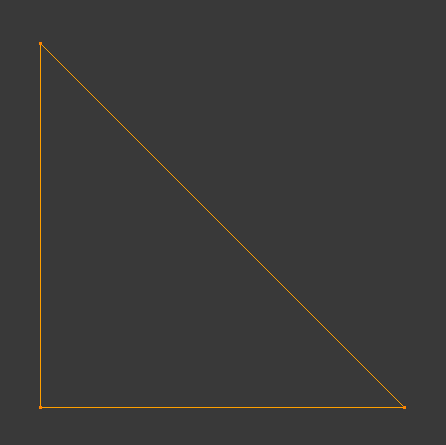
\includegraphics[width=\linewidth]{tex/img/ch03/Basics02_Edges.png}
    \subcaption{Edges}
    \label{fig:3d-edges}
\endminipage\hfill
\minipage{0.25\textwidth}%
    
\includegraphics[width=\linewidth]{tex/img/ch03/Basics03_Faces.png}
    \subcaption{Face}
    \label{fig:3d-face}
\endminipage
\minipage{0.25\textwidth}%
    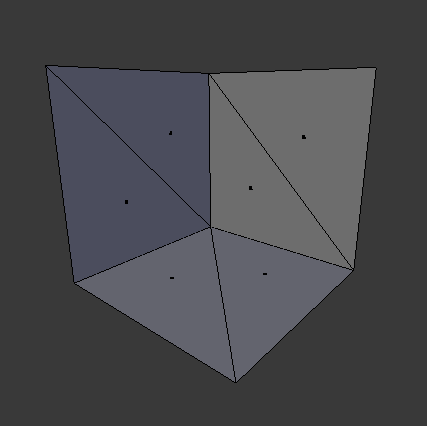
\includegraphics[width=\linewidth]{tex/img/ch03/Basics04_Meshes.png}
    \subcaption{Mesh}
    \label{fig:3d-mesh}
\endminipage
\captionof{figure}{Construction of a mesh}
\end{figure}

\paragraph{Materials} \textit{Textures} are images that are mapped to meshes for various uses. They can be used to encolor a mesh, manipulate its vertices height (\textit{Heightmap})\cite{UnityDocHeightmap} and simulate bumps (\textit{Normalmap}\cite{UnityDocNormalmap}\cite{Cohen:1998:AS:280814.280832}\cite{745285}) and reflections (\textit{Specularmap})\cite{UnityDocSpecularmap}.\\
\textit{UV-maps}.
Mapping textures to meshes requires a \textit{UV-map}

\begin{center}
\noindent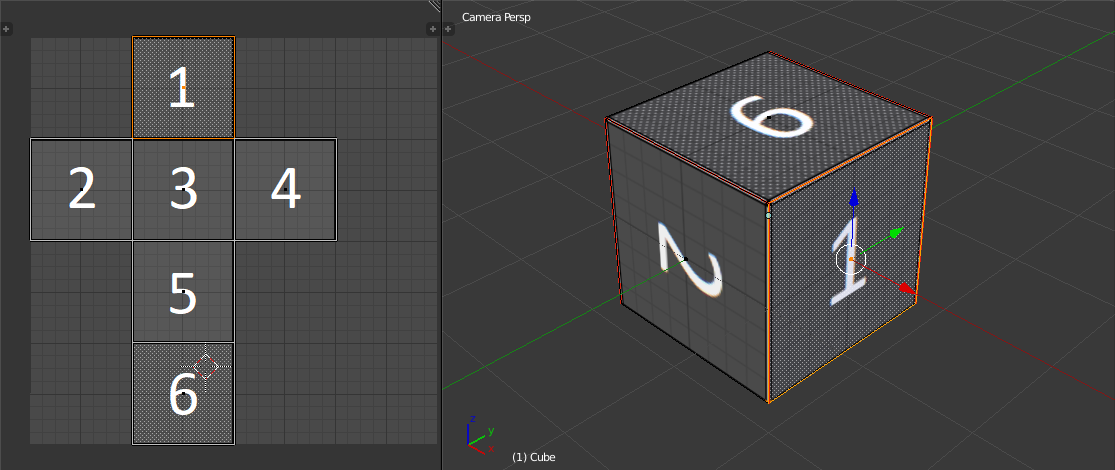
\includegraphics[width=12cm]{tex/img/ch03/CubeUVMapping.png}
\captionof{figure}{UV-map of a cube on top of a texture (l) and the same texture being applied to a cube (r) using the same UV-map where the face showing a "1" is highlighted.}
\label{fig:3d-cube-uv-mapping}
\end{center}

\subsection{Rendering}
Raytracing \cite{Plemenos2010} vs Rasterization [TBD]
Post-Processing [TBD]

%- Definition
   %- Techniques
%- Photorealism (Physics)

\subsection{Blender}
%- Why this one? (free, active development, support, cross-platform)
[TBD]

% //////////////////////////////////////////////////
\section{Game Engines}
Definition, Overview, Concepts (Entity Component System, Asset Bundles) [TBD]
%- Definition
%- Overview
%- Concepts

\subsection{Cry Engine}

\subsection{Source Engine}

\subsection{Unreal Engine}

\subsection{Unity}
%- Why this one? (free, cross-platform, simple development due to C#)
%- Entity Component System (behaviours)